\Section{theory}{General theory}

%In this section, we show how we can use pruning to obtain a sound analysis which
%is complete with respect to a given abstraction.
We first describe the core
idea behind pruning (\refsec{oneStep}) and then show how it can be used in the
Prune-Refine (\PR) algorithm (\refsec{algorithm}).

%%%%%%%%%%%%%%%%%%%%%%%%%%%%%%
\Subsection{oneStep}{Pruning}

Recall that the central operation of a static analysis is $\bP$, which serves two roles: (i)
determining if the query is proven (when $\bP$ returns $\emptyset$); and (ii)
returning the subset of relevant input tuples.
The following theorem provides the key equation that drives everything in this paper (see \refapp{proofs} for the proof):

\begin{theorem}[Pruning is sound and complete]
\label{thm:master}
Let $\alpha$ and $\beta$ be two abstractions such that $\beta \preceq \alpha$
($\beta$ is coarser than $\alpha$).
Then for any set of concrete input tuples $X$, we have:
\begin{align}
\label{eqn:master}
\boxed{
\bP(\alpha(X)) = \bP(\alpha(X) \cap \alpha(\bP(\beta(X)))).
}
\end{align}
\end{theorem}

The left-hand side of \refeqn{master} corresponds to running the analysis with respect to $\alpha$.
The right-hand side corresponds to first pruning the input tuples $X$
with $\beta$ and then running the analysis with $\alpha$.
The theorem states that the two procedures obtain identical results.
The significance of this is that the right-hand side is often a much cheaper
way to compute the left-hand side.

Let us decipher \refeqn{master} a bit more.
On the right-hand side,
the abstract input tuples $\beta(X)$
are fed into the Datalog solver which computes $\bP(\beta(X))$,
which is the subset of input tuples, namely those that participate in any derivation of the abstract query tuple $\beta(\xo)$.
These relevant tuples are then refined via $\alpha$ to yield a set of tuples which are used to prune $\alpha(X)$.
The resulting subset is fed into the analysis $\bP$.
On the left-hand side, $\bP(\alpha(X))$ is the result of directly running the analysis
on the abstract tuples $\alpha(X)$ without pruning.

% Generalization
To obtain some intuition behind pruning,
consider the following simpler idea:
first run the analysis with $\beta$; if the query is proven, stop and declare {\em proven}; otherwise, we run the analysis
with $\alpha$ and output that answer.
It is easy to see that this two-step procedure returns the same answer as just running $\alpha$,
because $\beta \preceq \alpha$ implies that if $\beta$ proves the query, then so does $\alpha$
(\refprop{soundness}).
\refeqn{master} can be thought of as an extension of this basic idea:
instead of using $\beta$ to just determine where the query tuple is proven,
we obtain more information, namely the set of input tuples that are relevant.

% Complexity
The complexity of an analysis is largely determined by the number of input
tuples.  Traditionally, the abstraction alone determines the set of input
tuples and thus also the complexity of the analysis.  In our case, however, the set
of input tuples is pruned along the way, so the abstraction only partially
determines the complexity.  As we will see later, with sufficient pruning of
the input tuples, we can use a very refined abstraction at a low cost.

%%%%%%%%%%%%%%%%%%%%%%%%%%%%%%
\Subsection{algorithm}{The Prune-Refine (\PR) algorithm}

\begin{figure}[t]
\begin{center} \scalebox{0.95}{\framebox{ \begin{minipage}{3.3in} % Begin model
\begin{center} Prune-Refine (\PR) Algorithm \end{center}
{\bf Input}: \\
\ind Sequence of abstractions: $\alpha_0 \preceq \alpha_1 \preceq \alpha_2 \preceq \cdots$ \\
\ind [Auxiliary abstractions: $\beta_t \preceq \alpha_t, t = 0, 1, 2, \dots$] \\
\ind $A_0 = \alpha_0(X)$, set of tuples \\
\\
For $t = 0, 1, 2, \dots$: \\
\ind [{\bf Pre-prune}: $A_t' \leftarrow A_t \cap \alpha_t(\bP(\beta_t(A_t)))$] \\
\ind {\bf Prune}: $\tilde A_t = \bP(A_t')$. If $\tilde A_t = \emptyset$: return {\em proven}. \\
\ind {\bf Refine}: $A_{t+1} = \alpha_{t+1}(\tilde A_t)$. \\
%\ind\ind\ind\ind\ind If $A_{t+1} = A_t$: return {\em not proven}.
\end{minipage} }} \end{center} % End model
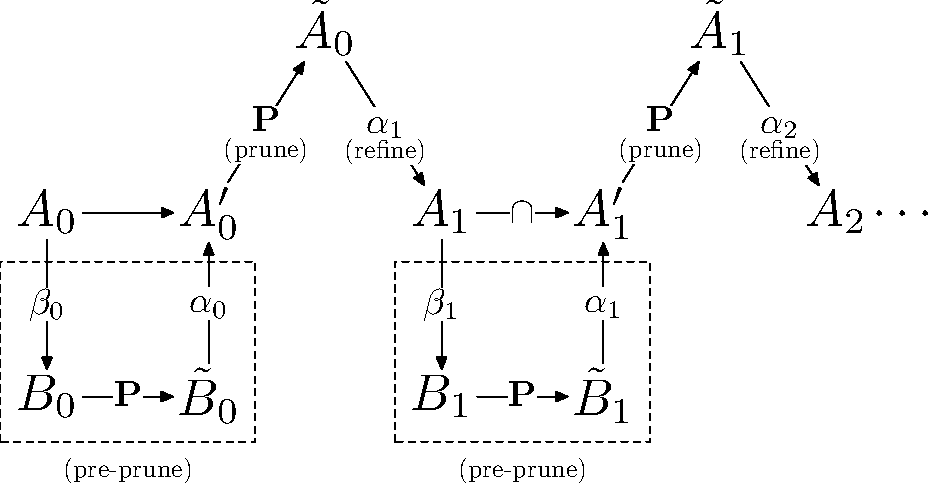
\includegraphics[scale=0.5]{figures/algorithm}
\caption{\label{fig:pseudocode} The pseudocode and the schema for the \PR\ algorithm.
The algorithm maintains a set of (abstract) input tuples which could be
involved in some derivation of the query $\xo$ and attempts to prune down this set.
The basic version, which excludes parts in square brackets,
simply alternates between pruning and refining.  The full version includes
a pre-pruning step using auxiliary abstractions in order to further reduce the
number of tuples.
}
\end{figure}

We now turn \refthm{master} into a full algorithm, which we call the
Prune-Refine (\PR) algorithm.  \reffig{pseudocode} shows the pseudocode
of the algorithm and a diagram showing the computation of the various abstract
input tuples computed.

% Basic
This algorithm essentially applies \refeqn{master} repeatedly.
We first present a simplified version of the algorithm which
ignores the pre-pruning step (we take $A_t = A_t'$).
We are given a sequence of successively finer abstractions $\alpha_0, \alpha_1, \dots$,
and an input set of abstract tuples $A_0$, which is computed
under the initial abstraction $\alpha_0$.  Then the algorithm alternates between a pruning step
and a refining step, always maintaining only the abstract tuples
that could participate in a derivation of the query tuple $\xo$.
On iteration $t$, our current input tuples $A_t$ are first pruned to $\tilde A_t$ using $\bP$;
this is subsequently refined to $A_{t+1}$.
% Example
\reffig{graphIters} shows an example of running this algorithm on the graph
example from \reffig{graphExample}; the first pruning step is shown in
\reffig{graphDerivation}.

\Fig{figures/graphIters}{0.3}{graphIters}{
The abstract input tuples computed by
the \PR\ algorithm on the graph example from \reffig{graphExample} (without pre-pruning),
where the abstraction $\alpha_t$ maps $c$ to all paths that match $c$ on the first $t+1$ nodes.
Notation: $c*$ denotes the set of all paths with prefix $c$.
During the first pruning step, $\ext(2,\vec{0}*,\vec{2}*)$ is pruned from $A_0$,
yielding $\tilde A_0$.  In the refine step, we expand $\vec{1}*$ to $\{ \vec{1} \}$ and $\vec{10}*$,
resulting in an extra tuple.  In the second pruning step, we prove the query
(pruning everything).
}

% Pre-pruning
Now we discuss pre-pruning.  Pre-pruning requires the user to provide
another sequence of successively finer abstractions $\beta_0, \beta_1, \dots$
which are coarser than $\alpha_0, \alpha_1, \dots$, respectively.
These abstractions will also be used to prune the input tuples.
The idea is that before refining $A_t$ to $A_{t+1}$,
we perform two steps of pruning:
(i) first using $\beta_t$ during pre-pruning step, and then
(ii) using $\alpha_t$ during the main pruning step.
Pre-pruning does not affect the output of the pruning step ($\tilde A_t$);
the purpose is solely to make the pruning step faster.
One way to obtain the auxiliary abstractions is via
compositions with another abstraction $\hclass$: $\beta_t = \alpha_t \circ \hclass$.
Intuitively, $\hclass$ should neither be too coarse nor too fine.
If $\hclass$ is no abstraction, then pre-pruning is equivalent to running the pruning step;
if $\hclass$ is the trivial abstraction, pre-pruning will be fast but nothing will be pre-pruned.
A rule of thumb is that $\hclass$ should be complementary to $\alpha_t$
(we will see examples in \refsec{abstractions}).

\refthm{algorithm} states that the \PR\ algorithm is both
sound and complete.  In other words, pruning has no impact on our answer to a
query---we just compute it more efficiently.
The proof is given in \refapp{proofs} and uses \refthm{master}.

\begin{theorem}[Correctness of the \PR\ algorithm]
\label{thm:algorithm}
At iteration $t$,
the incrementally pruned abstraction $A_t$ is equivalent
to the full abstraction $\alpha_t(X)$ (formally, $\bP(\alpha_t(X)) = \bP(A_t)$).
If the algorithm returns ``proven,'' then $\bP(X) = \emptyset$ (the query is actually false).
\end{theorem}
